%
%                  Politecnico di Milano
%
%          Gruppo: AM34
%            A.A.: 2022/2023
%
% Ultima modifica: 27/05/2023
%
%     Descrizione: Prova Finale (Progetto) di Ingegneria del Software - A.A. 2022/23
%                  Diapositive di accompagnamento alla presentazione finale
%

\documentclass[aspectratio=1610,10.5pt]{beamer} % Beamer (presentazione, con font a dimensione 10.5 e aspect ratio 16:10)

\usepackage[T1]{fontenc} % codifica dei font
\usepackage[utf8]{inputenc} % lettere accentate da tastiera
\usepackage[english,italian]{babel} % lingua del documento
\usepackage{lipsum} % genera testo fittizio
\usepackage{url} % per scrivere gli indirizzi Internet e/o di riferimento nella pagina

\usetheme{Frankfurt} % tema 1

% \usetheme{Boadilla} % tema 2

% \usetheme{Darmstadt} % tema 3

\usecolortheme{default} % tema colori 1 (default)

% \usecolortheme{rose} % tema colori 2

% \usecolortheme{whale} % tema colori 3

\setbeamersize{text margin left=2mm, text margin right=2mm} % margine di pagina

\setbeamertemplate{headline}{} % rimuove la barra di navigazione dall'intestazione
\setbeamertemplate{footline}[frame number] % numero di pagina in piè di pagina
\setbeamertemplate{navigation symbols}{} % rimuove simboli di navigazione
\setbeamercovered{invisible} % blocchi ancora da mostrare invisibili, esiste anche transparent

\usepackage[hidelinks]{hyperref} % per modificare il comportamento dei collegamenti ipertestuali (+ leva colore attorno)

\usepackage{graphicx} % per inserire immagini

\usepackage{blkarray} % per inserire blocchi Beamer

\usepackage{tikz} % pacchetto per la produzione di diagrammi
\usetikzlibrary{automata, positioning, arrows} % librerie per il tracciamento di ASF/FSM

\usepackage[outputdir=../auxil]{minted}
\usepackage{wasysym} % per colorazione automatica del codice (installare pygments da Homebrew)
% \usepackage{pythonhighlight} % per Python

\hypersetup{ % metadati di titolo e autore nel PDF
    pdftitle={Prova Finale di Ingegneria del Software - A.A. 2022/23},
    pdfauthor={Andrea Caravano - Biagio Cancelliere - Alessandro Cavallo - Allegra Chiavacci}
}

\begin{document}
    % Pagina del titolo
    \title{\textbf{Prova Finale (Progetto) di Ingegneria del Software}}
    \author{A.A. 2022/23\\Andrea Caravano\and Biagio Cancelliere\and Alessandro Cavallo\and Allegra Chiavacci}
    \institute{Gruppo AM34 - Scaglione A-E (prof. Margara)}
    \date{5 luglio 2023}
    \titlegraphic{\includegraphics[height=1.5cm]{../res/logo-polimi}}

    % logo in basso a destra
    %\logo{\includegraphics[height=%
    %0.15\textheight]{../res/logo-polimi}}

    % Creazione pagina del titolo
    \begin{frame}
        \titlepage
    \end{frame}

    % indice del documento (relativo alle sezioni e non ai frame)
    %\begin{frame}{Indice}
    %    \tableofcontents
    %\end{frame}

    \logo{} % rimuove il logo dalle slide successive


    \section{Fasi dello sviluppo}\label{sec:fasi-dello-sviluppo}
    \begin{frame}{Fasi dello sviluppo}
        \begin{columns}
            \begin{column}{0.54\textwidth}
                \begin{block}{Fasi dello sviluppo}
                    \begin{center}
                        \begin{tabular}{|c|c|}
                            \hline
                            {\small Diagramma UML iniziale del model\par}                & \checked \\
                            \hline
                            {\small Diagramma UML iniziale di model e controller\par}    & \checked \\
                            \hline
                            {\small Peer review n. 1\par}                                & \checked \\
                            \hline
                            {\small Implementazione e testing di model e controller\par} & \checked \\
                            \hline
                            {\small Documentazione del protocollo di comunicazione\par}  & \checked \\
                            \hline
                            {\small Peer review n. 2\par}                                & \checked \\
                            \hline
                            {\small Implementazione del protocollo di comunicazione\par} & \checked \\
                            {\small (RMI + Socket)\par}                                  &          \\
                            \hline
                            {\small GUI in RMI\par}                                      & \checked \\
                            \hline
                            {\small GUI in Socket\par}                                   & \checked \\
                            \hline
                            {\small JavaDoc\par}                                         & \checked \\
                            \hline
                            {\small Diagrammi UML finali\par}                            & \checked \\
                            \hline
                            {\small Rapporto sui test di unità\par}                      & \checked \\
                            \hline
                            {\small Funzionalità avanzate\par}                           & \checked \\
                            \hline
                            {\small Produzione pacchetto esegubile\par}                  & \checked \\
                            \hline
                        \end{tabular}
                    \end{center}
                \end{block}
            \end{column}
            \begin{column}{0.4\textwidth}
                \begin{block}{Funzionalità avanzate}
                    \begin{center}
                        \begin{tabular}{|c|c|}
                            \hline
                            {\small Partite multiple\par} & \checked \\
                            \hline
                            {\small Persistenza\par}      & \checked \\
                            \hline
                        \end{tabular}
                    \end{center}
                \end{block}
                \begin{block}{Extra}
                {\small È disponibile un Server reale a cui collegarsi tramite il client Socket via TCP.\par}
                    \hfill \linebreak
                    {\small Esso è ospitato presso \texttt{myshelfie.andreacaravano.net} alla \texttt{porta 3435}.\par}
                    \hfill \linebreak
                    {\small Viene offerta una \href{http://myshelfie.andreacaravano.net/log/}{piattaforma di logging} e di \href{http://myshelfie.andreacaravano.net/games-persistency/}{persistenza delle partite} in corso.\par}
                \end{block}
            \end{column}
        \end{columns}
    \end{frame}


    \section{Diagramma UML iniziale di Model e Controller}\label{sec:diagramma-uml-iniziale-di-model-e-controller}
    \begin{frame}{Diagramma UML iniziale di Model e Controller}
        \includegraphics[height=8.9cm]{../res/uml-iniziale}
    \end{frame}


    \section{Diagramma UML finale di Model e Controller}\label{sec:diagramma-uml-finale-di-model-e-controller}
    \begin{frame}{Diagramma UML finale di Model e Controller - di alto livello}
        \begin{center}
            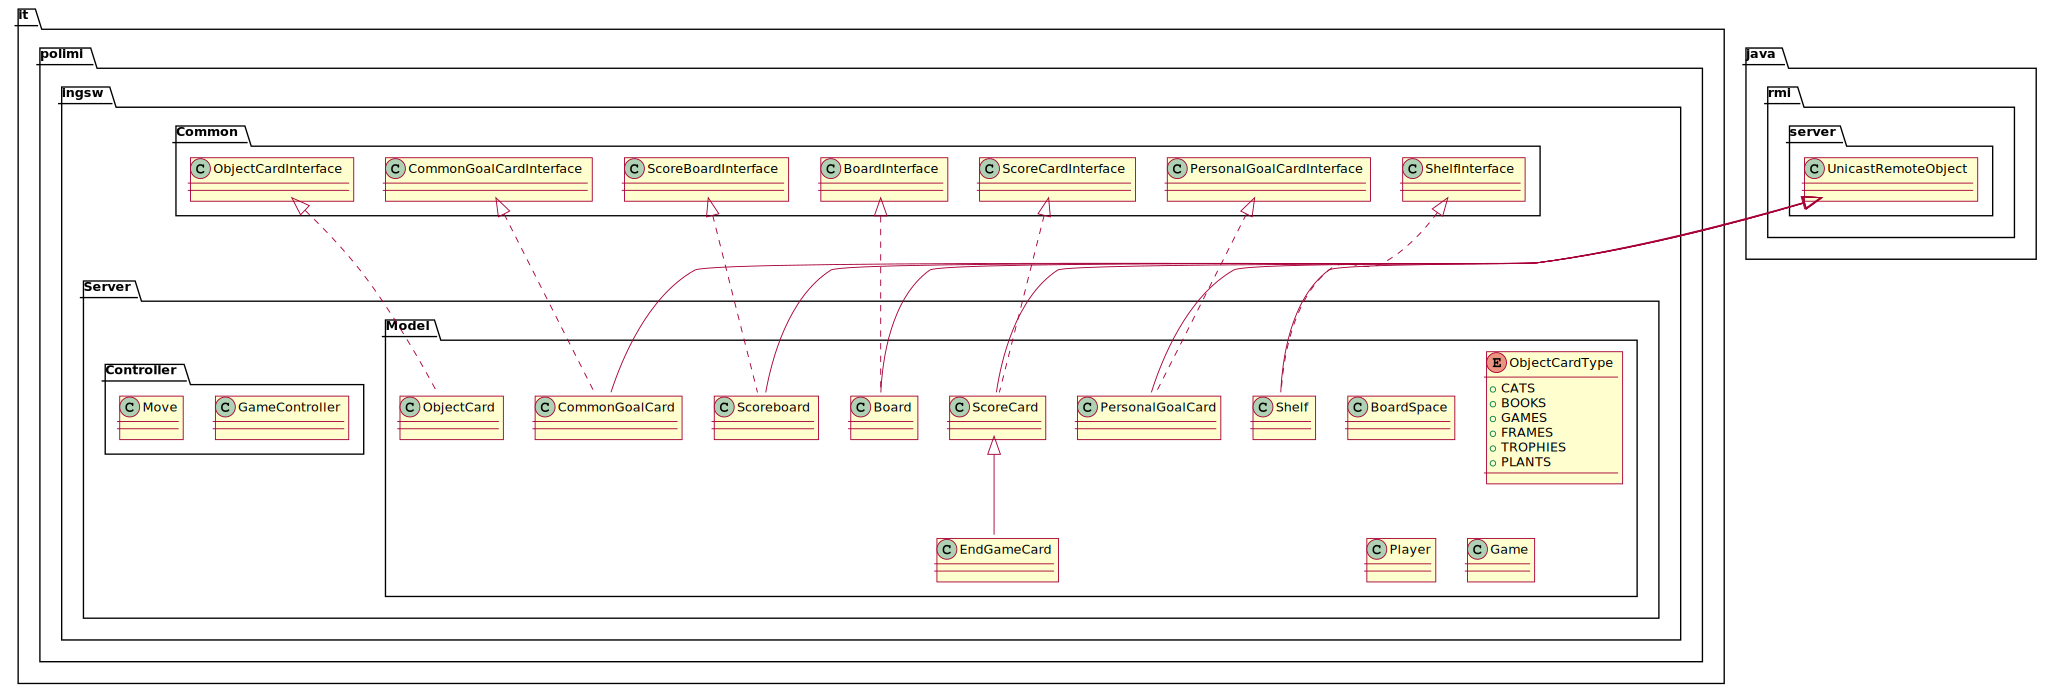
\includegraphics[height=5.3cm]{../res/abstract-model-controller}
        \end{center}
    \end{frame}


    \section{Diagramma UML finale di Server e Client}\label{sec:diagramma-uml-finale-di-server-e-client}
    \begin{frame}{Diagramma UML finale di Server e Client - di alto livello}
        \begin{center}
            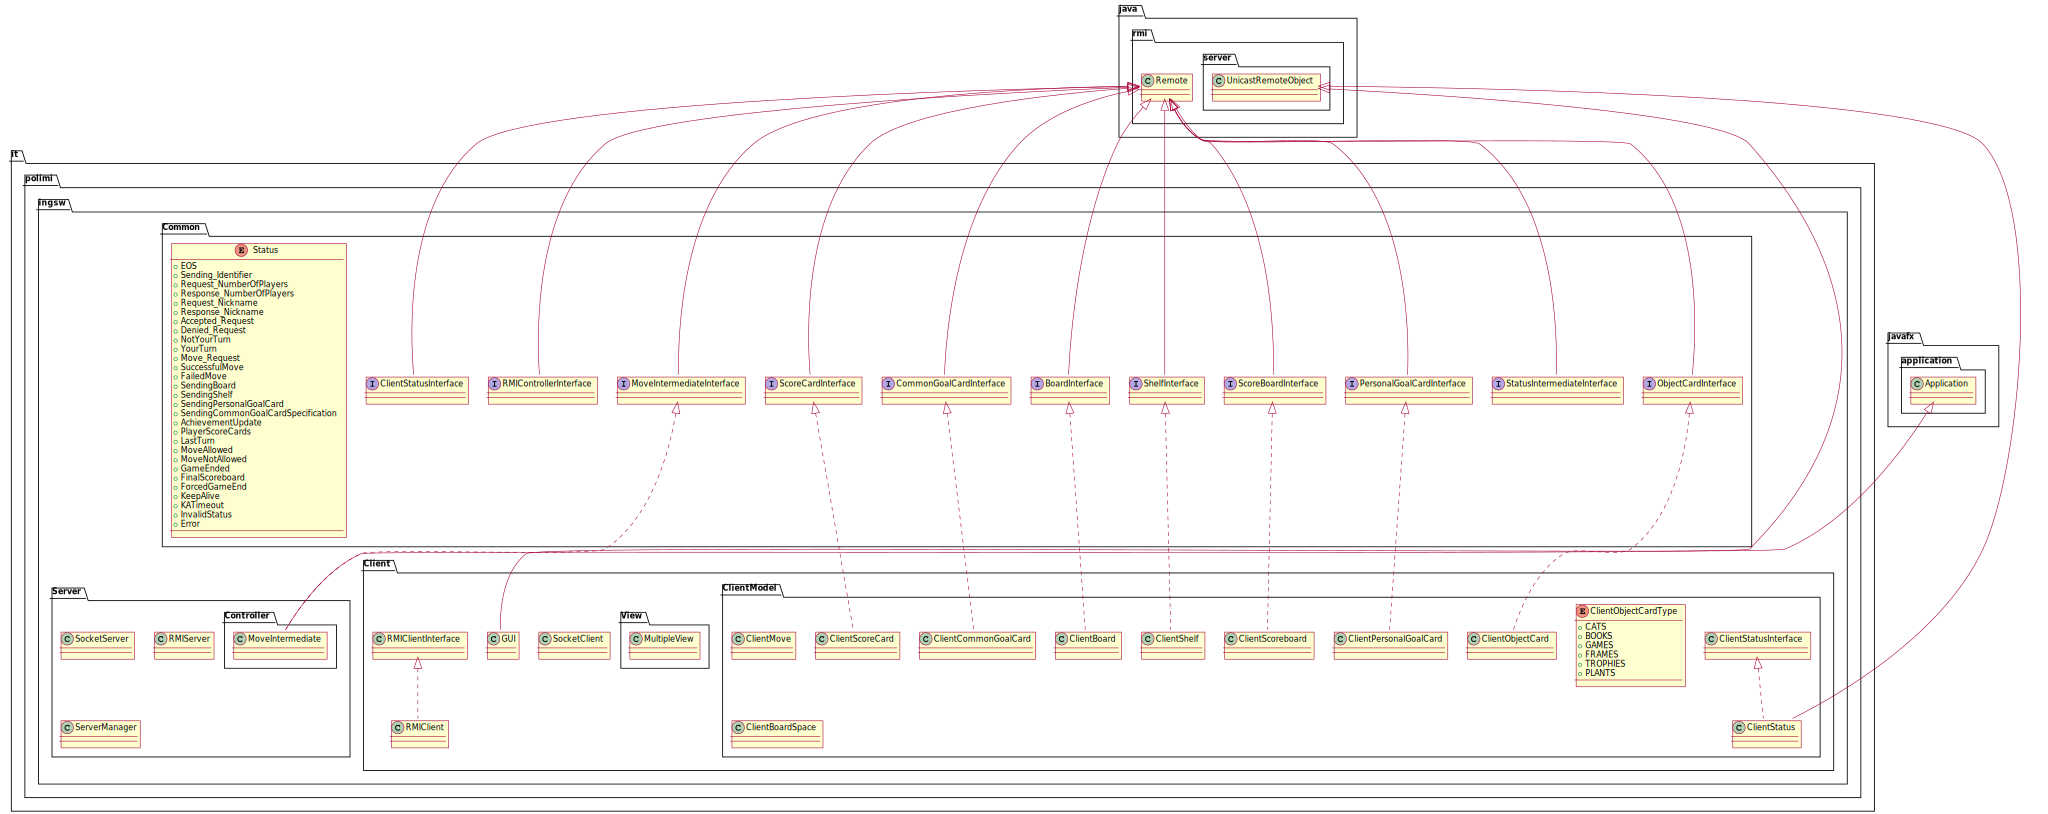
\includegraphics[height=6.3cm]{../res/abstract-server-client}
        \end{center}
    \end{frame}


    \section{Un esempio di scambio - Socket}\label{sec:un-esempio-di-scambio---socket}
    \begin{frame}{Un esempio di scambio - Socket}
        \begin{center}
            \includegraphics[height=8.7cm]{../res/socket-2}
        \end{center}
    \end{frame}


    \section{Un esempio di scambio - RMI}\label{sec:un-esempio-di-scambio---rmi}
    \begin{frame}{Un esempio di scambio - RMI}
        \begin{center}
            \includegraphics[height=8.9cm]{../res/rmi-2}
        \end{center}
    \end{frame}


    \section{Fasi dello sviluppo}\label{sec:fasi-dello-sviluppo-2}
    \begin{frame}{Fasi dello sviluppo}
        \begin{columns}
            \begin{column}{0.54\textwidth}
                \begin{block}{Fasi dello sviluppo}
                    \begin{center}
                        \begin{tabular}{|c|c|}
                            \hline
                            {\small Diagramma UML iniziale del model\par}                & \checked \\
                            \hline
                            {\small Diagramma UML iniziale di model e controller\par}    & \checked \\
                            \hline
                            {\small Peer review n. 1\par}                                & \checked \\
                            \hline
                            {\small Implementazione e testing di model e controller\par} & \checked \\
                            \hline
                            {\small Documentazione del protocollo di comunicazione\par}  & \checked \\
                            \hline
                            {\small Peer review n. 2\par}                                & \checked \\
                            \hline
                            {\small Implementazione del protocollo di comunicazione\par} & \checked \\
                            {\small (RMI + Socket)\par}                                  &          \\
                            \hline
                            {\small GUI in RMI\par}                                      & \checked \\
                            \hline
                            {\small GUI in Socket\par}                                   & \checked \\
                            \hline
                            {\small JavaDoc\par}                                         & \checked \\
                            \hline
                            {\small Diagrammi UML finali\par}                            & \checked \\
                            \hline
                            {\small Rapporto sui test di unità\par}                      & \checked \\
                            \hline
                            {\small Funzionalità avanzate\par}                           & \checked \\
                            \hline
                            {\small Produzione pacchetto esegubile\par}                  & \checked \\
                            \hline
                        \end{tabular}
                    \end{center}
                \end{block}
            \end{column}
            \begin{column}{0.4\textwidth}
                \begin{block}{Funzionalità avanzate}
                    \begin{center}
                        \begin{tabular}{|c|c|}
                            \hline
                            {\small Partite multiple\par} & \checked \\
                            \hline
                            {\small Persistenza\par}      & \checked \\
                            \hline
                        \end{tabular}
                    \end{center}
                \end{block}
                \begin{block}{Extra}
                {\small È disponibile un Server reale a cui collegarsi tramite il client Socket via TCP.\par}
                    \hfill \linebreak
                    {\small Esso è ospitato presso \texttt{myshelfie.andreacaravano.net} alla \texttt{porta 3435}.\par}
                    \hfill \linebreak
                    {\small Viene offerta una \href{http://myshelfie.andreacaravano.net/log/}{piattaforma di logging} e di \href{http://myshelfie.andreacaravano.net/games-persistency/}{persistenza delle partite} in corso.\par}
                \end{block}
            \end{column}
        \end{columns}
    \end{frame}
\end{document}